% Chapter Template

\chapter{Ensayos y resultados} % Main chapter title

\label{Chapter4} % Change X to a consecutive number; for referencing this chapter elsewhere, use \ref{ChapterX}

%----------------------------------------------------------------------------------------
%	SECTION 1
%----------------------------------------------------------------------------------------

\section{Laboratorio remoto}
\label{sec:lab}

\begin{figure}[htbp]
	\centering
	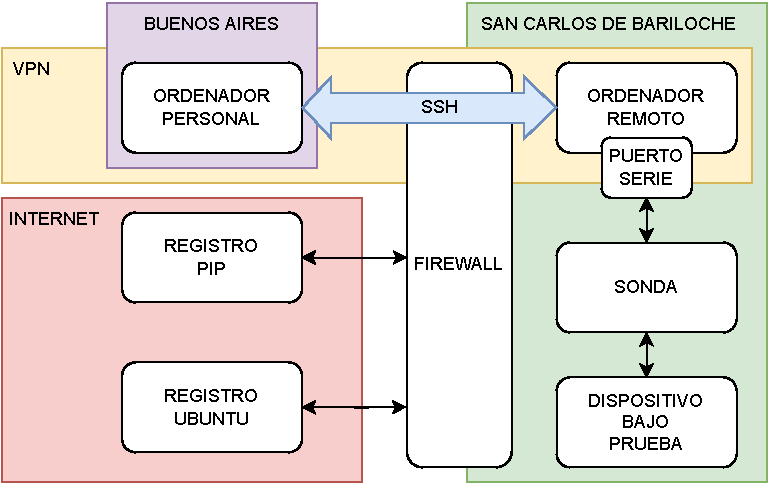
\includegraphics[width=\textwidth]{./Figures/vpn.pdf}
    \caption{Diagrama en bloques del laboratorio remoto.}
	\label{fig:remotelab}
\end{figure}

\begin{table}[h]
	\centering
	\caption[]{}

	\begin{tabular}{l c}    
		\toprule
        \textbf{Funcionalidad}             & \textbf{Nivel de servicio} \\
		\midrule
		Carga de binarios en DUT           & ++  \\		
		Comunicación con registro PIP      & +++ \\
		Comunicación con registro Ubuntu   & +++ \\
		Comunicación con debug access port & +++ \\
		Comunicación con UART              & +   \\
		\bottomrule
		\hline
	\end{tabular}
	\label{tab:funcionalidades}
\end{table}

\section{Ensayos de inyector}
\label{sec:testinyector}

\begin{figure}[htbp]
	\centering
	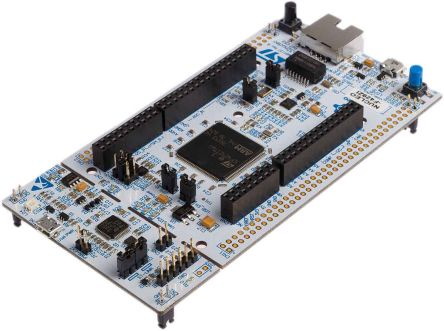
\includegraphics[width=0.8\textwidth]{./Figures/alternativo.jpg}
    \caption{Dispositivo alternativo \emph{NUCLEO-F429ZI}.}
	\label{fig:alternativo}
\end{figure}

\begin{table}[h]
	\centering
	\caption[Resumen de ensayos]{Resumen de ensayos}

	\begin{tabular}{l c c c}    
		\toprule
        \textbf{Ensayo}                 & \textbf{Lab. local} & \textbf{Lab. remoto} & \textbf{DUT alterno} \\
		\midrule
		Escritura SDRAM                 & +++                 & +++                  & +++ \\
		Escritura registros CORE        & +++                 & +++                  & +++ \\
		Funcionalidades extras          & ++                  & ++                   & +++ \\
		Halt CORE                       & +++                 & +++                  & +++ \\
		Lectura SDRAM                   & +++                 & +++                  & +++ \\
		Lectura registros CORE          & +++                 & +++                  & +++ \\		
		Uso concurrente de puerto serie & +++                 & +                    & +++ \\
        Resume CORE                     & +++                 & +++                  & +++ \\
		\bottomrule
		\hline
	\end{tabular}
	\label{tab:resensayos}
\end{table}

\section{Validación con el cliente}
\label{sec:validacion}

\begin{table}[h]
	\centering
	\caption[Resumen de la validación con el cliente]{Resumen de la validación con el cliente}

	\begin{tabular}{l c}    
		\toprule
        \textbf{Expectativas}     & \textbf{Cumplimiento} \\
		\midrule
		Acceso a memoria          & +++                   \\
		Acceso al CORE            & +++                   \\
		Biblioteca de ensayos     & +++                   \\		
		Capacidad de bit-flip     & +++                   \\
		Configuración del sistema & +++                   \\
		Distribución de errores   & +++                   \\
		Validación de periféricos & +++                   \\
        Generación de reportes    & +++                   \\
		\bottomrule
		\hline
	\end{tabular}
	\label{tab:validacion}
\end{table}
